\label{sec:testnum}
\begin{remark*}

    La fonction de la question 32(b) est incluse dans le code fourni dans l'\hyperref[sec:fonctions]{annexe B}. Le reste du code lié à cette partie est intégré au \hyperref[sec:main]{main}.

\end{remark*}

\begin{reponse}{30}
\begin{center}
    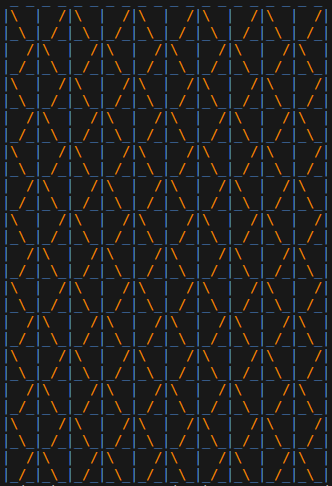
\includegraphics[width=0.4\linewidth]{maillage.png}
    \captionof{figure}{Affichage du maillage $N \times M = 10 \times 14$ dans le terminal}
\end{center}
\end{reponse}

%%%%%%%%%%%%%%%%%%%%%%%%%%%%%%%%%%%%%%%%%%%%%%%%%%%%%%%%%%%%%%%%%%%%%%%%%%%%%%%%

\begin{reponse}{31}

Soient $h_1 = \frac{2a}{N}, h_2 = \frac{2b}{M}$ et $h=\max(h_1,h_2)$. Soit $(x,y) \in \Omega$ quelconque. Alors en particulier, $x \in \, ]-a,a \,[$ et $y \in \, ]-b,b\,[$. Ainsi,

\begin{align*}
    x \in \, ]-a,a \,[ \quad & \Longleftrightarrow \quad -a<x<a \quad \Longleftrightarrow \quad 0<x+a<2a \\
    &\Longleftrightarrow \quad 0 < \frac{x+a}{h_1} < N \quad \Longleftrightarrow \quad 0<i<N.
\end{align*}

D'où $i \leq N-1$. De la même manière,

\begin{align*}
    y \in \, ]-b,b \,[ \quad & \Longleftrightarrow \quad -b<y<b \quad \Longleftrightarrow \quad 0<y+b<2b \\
    &\Longleftrightarrow \quad 0 < \frac{y+b}{h_2} < M \quad \Longleftrightarrow \quad 0<j<M.
\end{align*}

Ce qui donne $j \leq M-1$. \\ \\
Par définition de la partie entière,

\begin{align*}
    i = \operatorname{E}\left[\frac{x+a}{h_1}\right] & \Longrightarrow i \leq \frac{x+a}{h_1} < i+1 \\
    & \Longleftrightarrow \quad ih_1 \leq x+a \leq (i+1)h_1 \\ \\
    &\Longleftrightarrow \quad -a+ih_1 \leq x < -a+(i+1)h_1 \\ \\
    & \Longleftrightarrow \quad x_i \leq x < x_{i+1}.
\end{align*}

De manière analogue,

\begin{align*}
    j = \operatorname{E}\left[\frac{y+b}{h_2}\right] & \Longrightarrow j \leq \frac{y+b}{h_2} < j+1 \\
    & \Longleftrightarrow \quad jh_2 \leq y+b \leq (j+1)h_2 \\ \\
    & \Longleftrightarrow \quad -b+jh_2 \leq y < -b+(j+1)h_2 \\ \\
    & \Longleftrightarrow \quad y_j \leq y < y_{j+1}.
\end{align*}

On en déduit donc que $(x,y) \in [x_i,x_{i+1}[ \, \times \,  [y_j,y_{j+1}[$. Or $[x_i,x_{i+1}[ \, \times \,  [y_j,y_{j+1}[ \, \subset \,  T_l \cup T_{l+1}$. En effet, d'après la numérotation des noeuds que l'on a réalisé dans la partie 2, les sommets de $T_l$ et $T_{l+1}$ avec $l=(N+1)j+i$ sont respectivement $\{ \, (x_i,y_j), (x_i, y_{j+1}), (x_{i+1}, y_j) \, \}$ et $\{ \, (x_i,y_{j+1}), (x_{i+1}, y_{j+1}), (x_{i+1}, y_j) \, \}$ (ou bien $\{ \, (x_i,y_j), (x_i, y_{j+1}), (x_{i+1}, y_{j+1}) \, \}$ et $\{ \, (x_i,y_j), (x_{i+1}, y_{j+1}), (x_{i+1}, y_j) \, \}$ selon le sens de la partition du rectangle) :

\begin{center}
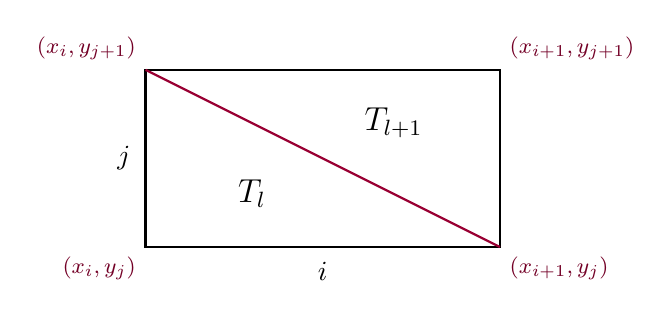
\begin{tikzpicture}[scale=2.5]
    \def\w{1.8}
    \def\h{0.9}
    \draw [thick] (0,0) rectangle (\w,\h);
    \draw [draw=purple!80!black, thick] (0,\h) -- (\w,0);
    \node [text=black, font=\large] at (\w*0.3, \h*0.3) {$\boldsymbol{T_{l}}$};
    \node [text=black, font=\large] at (\w*0.7, \h*0.7) {$\boldsymbol{T_{l+1}}$};
    \node [text=purple!60!black, font=\footnotesize, below left] at (0,0) {$(x_i,y_j)$};
    \node [text=purple!60!black, font=\footnotesize, below right] at (\w,0) {$(x_{i+1},y_j)$};
    \node [text=purple!60!black, font=\footnotesize, above left] at (0,\h) {$(x_i,y_{j+1})$};
    \node [text=purple!60!black, font=\footnotesize, above right] at (\w,\h) {$(x_{i+1},y_{j+1})$};
    \node [left=2pt] at (0, \h/2) {$j$};
    \node [below=2pt] at (\w/2, 0) {$i$};
\end{tikzpicture}
\end{center}

On a donc $(x,y) \in \, T_l \cup T_{l+1}$ et donc $(x,y) \in \, T_l$ ou $(x,y) \in \, T_{l+1}$.

\end{reponse}

%%%%%%%%%%%%%%%%%%%%%%%%%%%%%%%%%%%%%%%%%%%%%%%%%%%%%%%%%%%%%%%%%%%%%%%%%%%%%%%%

\begin{reponse}{32}

\textbf{(a)} D'après la question 3,

\[
    u^p(x,y) = \frac{\cos (m \pi x) \cos (m \pi y)}{2m^2\pi^2 +1}
\]

Pour simplifier l'écriture, on pose $C=\frac{1}{2m^2\pi^2 +1}$. On a d'une part

\[
    \frac{\partial u^p}{\partial x}(x,y) = -Cm\pi\sin(m \pi x)\cos(m\pi y),
\]

et d'autre part

\[
    \frac{\partial u^p}{\partial y}(x,y) = -Cm\pi\cos(m \pi x)\sin(m\pi y).
\]

On calcule ensuite les dérivées secondes :

\[
    \frac{\partial ^2u^p}{\partial x^2}(x,y) = -Cm^2\pi^2\cos (m\pi x)\cos(m\pi y) = -m^2\pi^2 u^p(x,y)
\]

et

\[
    \frac{\partial ^2u^p}{\partial y^2}(x,y) =-m^2\pi^2 u^p(x,y).
\]

On pose $\eta \, (x,y) = 1- \frac{\eta_0}{4}(x^2+y^2)$. Ainsi,

\[
    \frac{\partial}{\partial x}\left(\eta \frac{\partial u^p}{\partial x}\right)(x,y) = \frac{\eta_0x}{2}Cm\pi \sin(m \pi x) \cos(m \pi y) - m² \pi^2 u^p(x,y)\eta \, (x,y) := A(x,y)
\]

et

\[
        \frac{\partial}{\partial y}\left(\eta \frac{\partial u^p}{\partial y}\right)(x,y) = \frac{\eta_0x}{2}Cm\pi \cos(m \pi x) \sin(m \pi y) - m² \pi^2 u^p(x,y)\eta \, (x,y) := B(x,y).
\]

En reprenant l'équation (1) du sujet, avec $\lambda = 1$, on obtient alors

\begin{align*}
   & -\frac{\partial}{\partial x} \left( \eta \frac{\partial u^p}{\partial x}\right)(x,y) -\frac{\partial}{\partial y} \left( \eta \frac{\partial u^p}{\partial y}\right)(x,y) + \lambda u^p(x,y) = f(x,y) \\ \\
   \Longleftrightarrow \quad & f(x,y) = - A(x,y) - B(x,y) + u^p(x,y)
\end{align*}

En remplaçant $A(x,y)$ et $B(x,y)$ par leur expression donnée plus haut puis en factorisant, on obtient finalement :

\begin{align*}
    f(x,y) = -\frac{\eta_0 m \pi}{4m^2\pi^2 + 2}(x\sin(m\pi x)\cos(m\pi y)+ & y\cos(m\pi x)\sin(m\pi y)) \\
    & +(2m^2\pi^2\eta\,(x,y)+1)u^p(x,y).
\end{align*}

%%%%%%%%%%%%%%%%%%%%%%%%%%%%%%%%%%%%%%%%%%%%%%%%%%%%%%%%%%%%%%%%%%%%%%%%%%%%%%%%
\vspace{0.8em}
\textbf{(c)} En testant pour $m=1.$ et $N=M=2/h \in \{\,4,8,16,20,32,64,128 \,\}$, nous avons obtenu les erreurs relatives suivantes :

\begin{codeblock}
N e0 e1 e2
4 0.00137758 0.00137758 0.00137758
8 0.0425056 0.132984 0.0691583
16 0.00954852 0.0656942 0.022318
20 0.00602898 0.052484 0.0146806
32 0.00232045 0.032755 0.00590366
64 0.000575973 0.0163662 0.00149802
128 0.000143869 0.0081817 0.000378497
\end{codeblock}

\vspace{0.8em}

Avec le passage au log et un test sur un plus grand nombre de valeurs de $N$, cela nous a permis d'obtenir le graphe suivant :

\begin{center}
    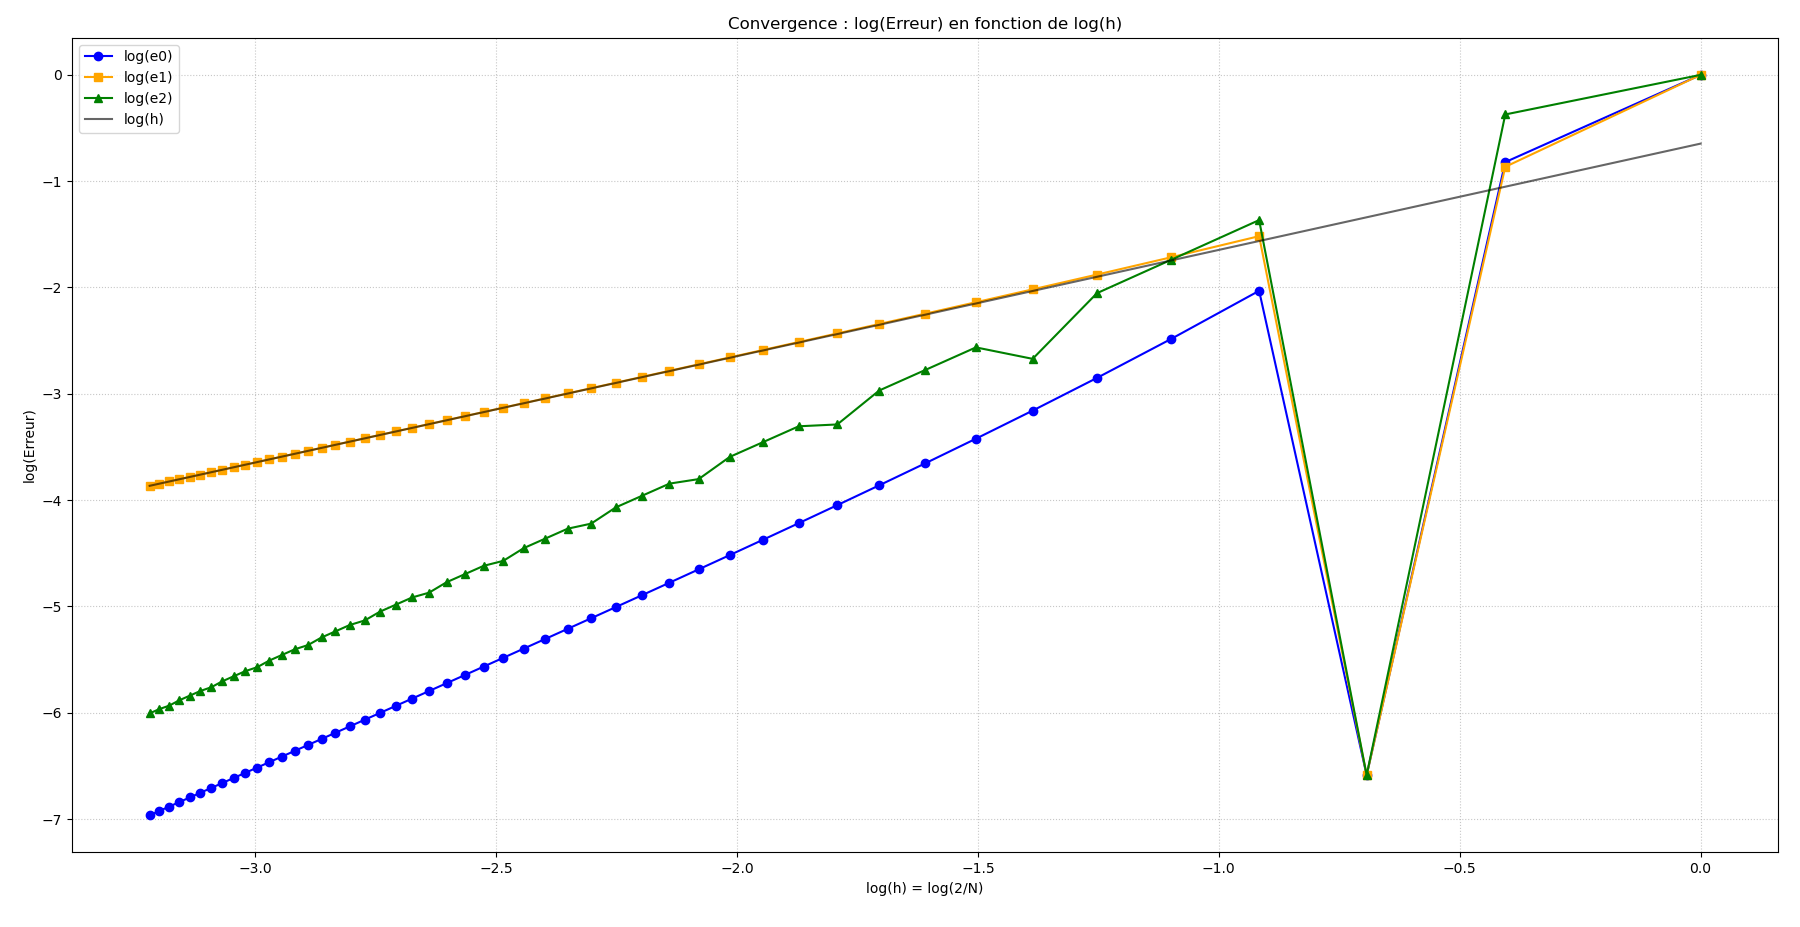
\includegraphics[width=1\linewidth]{erreurs.png}
    \captionof{figure}{Tracé des courbes d'erreurs}
\end{center}

\vspace{0.8em}

On remarque que pour $N=4$, l'erreur plonge, ce qui indique que la solution approchée correspond presque exactement à la solution réelle : les noeuds du maillage semblent donc coïncider avec les points de la solution exacte.

%%%%%%%%%%%%%%%%%%%%%%%%%%%%%%%%%%%%%%%%%%%%%%%%%%%%%%%%%%%%%%%%%%%%%%%%%%%%%%%%
\vspace{1.6em}
\textbf{(d)} A partir de la question 31, nous avons pu créer une fonction eval\_uh que nous avons évalué en 50 points pour différentes valeurs de $m$. En comparant avec la fonction log(h), nous avons obtenu les graphes suivants :

\begin{center}
    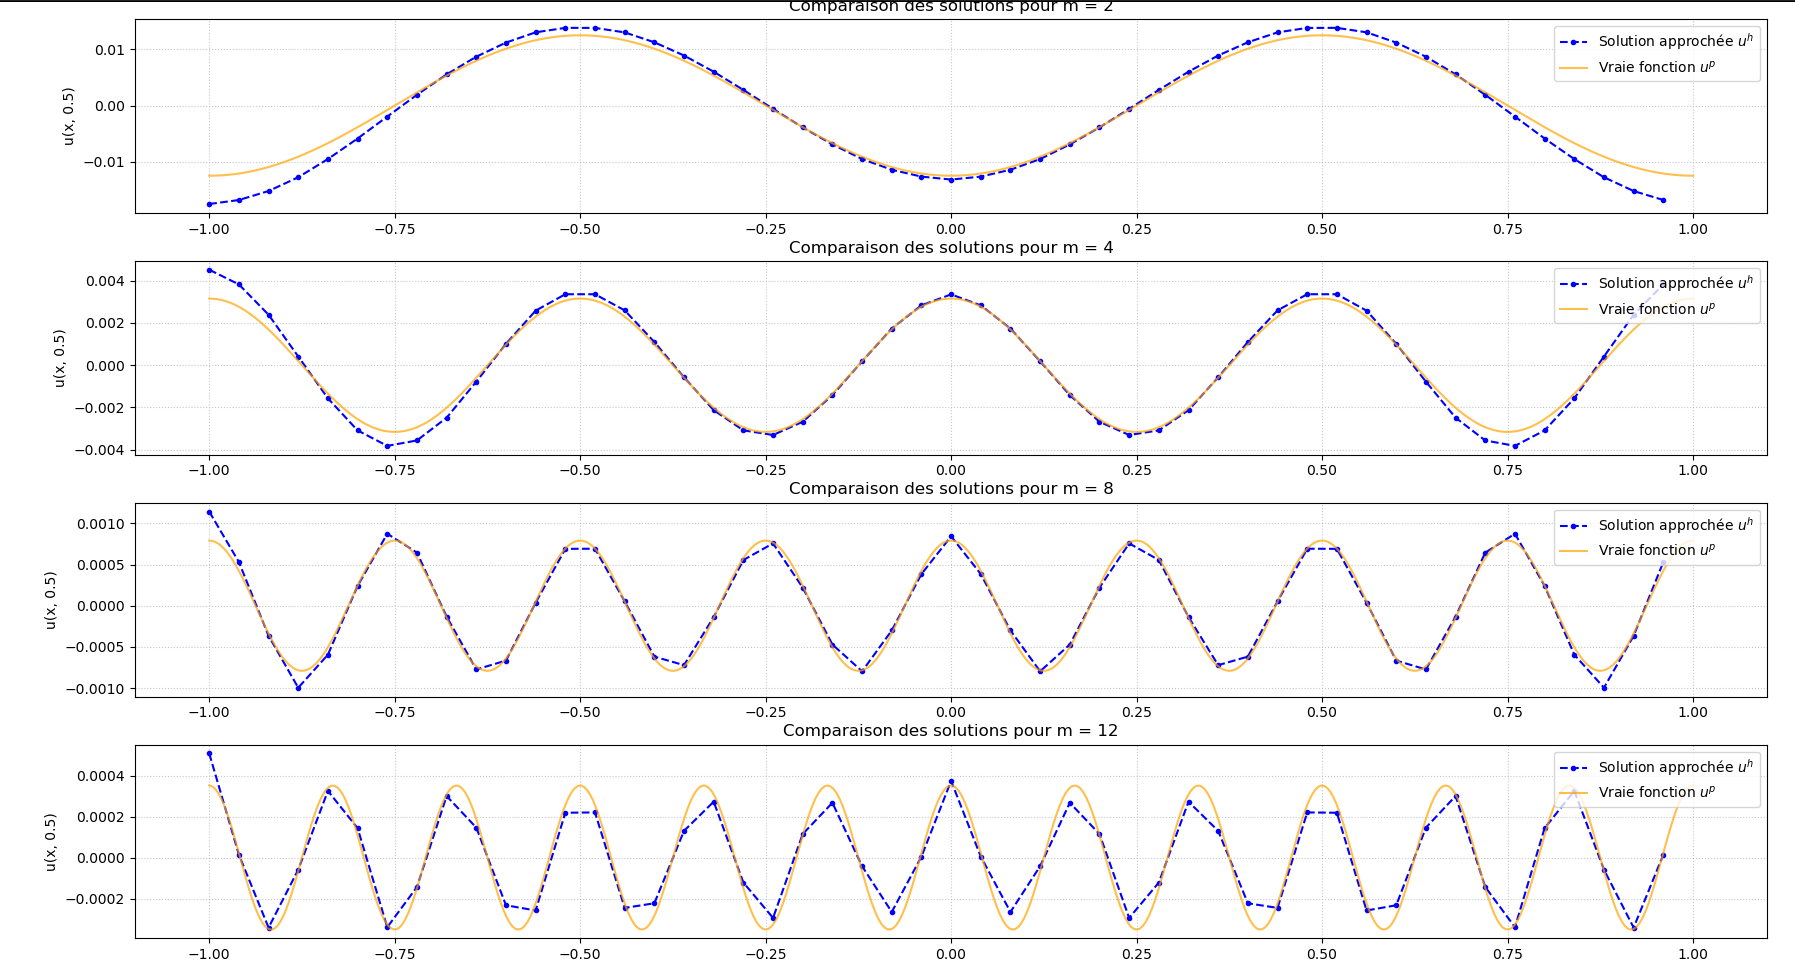
\includegraphics[width=1\linewidth]{graphes.png}
    \captionof{figure}{Tracé des courbes pour $x \in [-1,1]$}
\end{center}

\vspace{0.8em}

On observe que pour des petites valeurs de m ($2,4$) le maillage $N=32$ est suffisant, mais lorsque $m$ grandit, le maillage n'est plus assez fin pour capter les variations de la fonction, et donc l'erreur est bien plus grande.

\end{reponse}